%%%%%%%%%%%%%%%%%%%%%%%%%%%%%%%%%%%%%%%%%

\chapter{The LANL nEDM experiment}\label{chap:LANL_nEDM}

%%%%%%%%%%%%%%%%%%%%%%%%%%%%%%%%%%%%%%%%%

%%%%%%%%%%%%%%%%%%%%%%%%%%%%%%%%%%%%%%%%%

\section{Basics of an nEDM measurement}

%%%%%%%%%%%%%%%%%%%%%%%%%%%%%%%%%%%%%%%%%


%%%%%%%%%%%%%%%%%%%%%%%%%%%%%%%%%%%%%%%%%

\section{Overview of the LANL nEDM experiment}

%%%%%%%%%%%%%%%%%%%%%%%%%%%%%%%%%%%%%%%%%

At the Los Alamos National Laboratory (LANL), a solid deuterium (SD$_2$) based superthermal UCN source coupled to a spallation target has been providing UCN to experiments for the last 20 years. The UCN source (Sec.~\ref{sec:lanl_ucn_source}) has recently been upgraded to host a new nEDM experiment that will use Ramsey's method of separated oscillatory fields to search for the nEDM with an uncertainty goal of $\delta \gls*{d_n} = 2\times 10^{-27}$~$e\cdot\text{cm}$ (Sec.~\ref{sec:figure_of_merit}).

The finalized LANL nEDM experiment will include features such as \comment{further elaborates}:
%
\begin{enumerate}
    \item Two precession chambers \comment{to reduce the number of times B and E fields are flipped}
    \item Simultaenous spin analyzers
    \item An external array of optically pumped magnetometers
    \item A $\ce{^{199}Hg$ comagnetometer and external $\ce{^{199}Hg$ comagnetometers
\end{enumerate}

%%%%%%%%%%%%%%%%%%%%%%%%%%%%%%%%%%%%%%%%%

\subsection{Layout of experimental area}

%%%%%%%%%%%%%%%%%%%%%%%%%%%%%%%%%%%%%%%%%

(see Fig.~\ref{fig:AreaB_schematic})

\begin{figure}[htp]
    \centering
    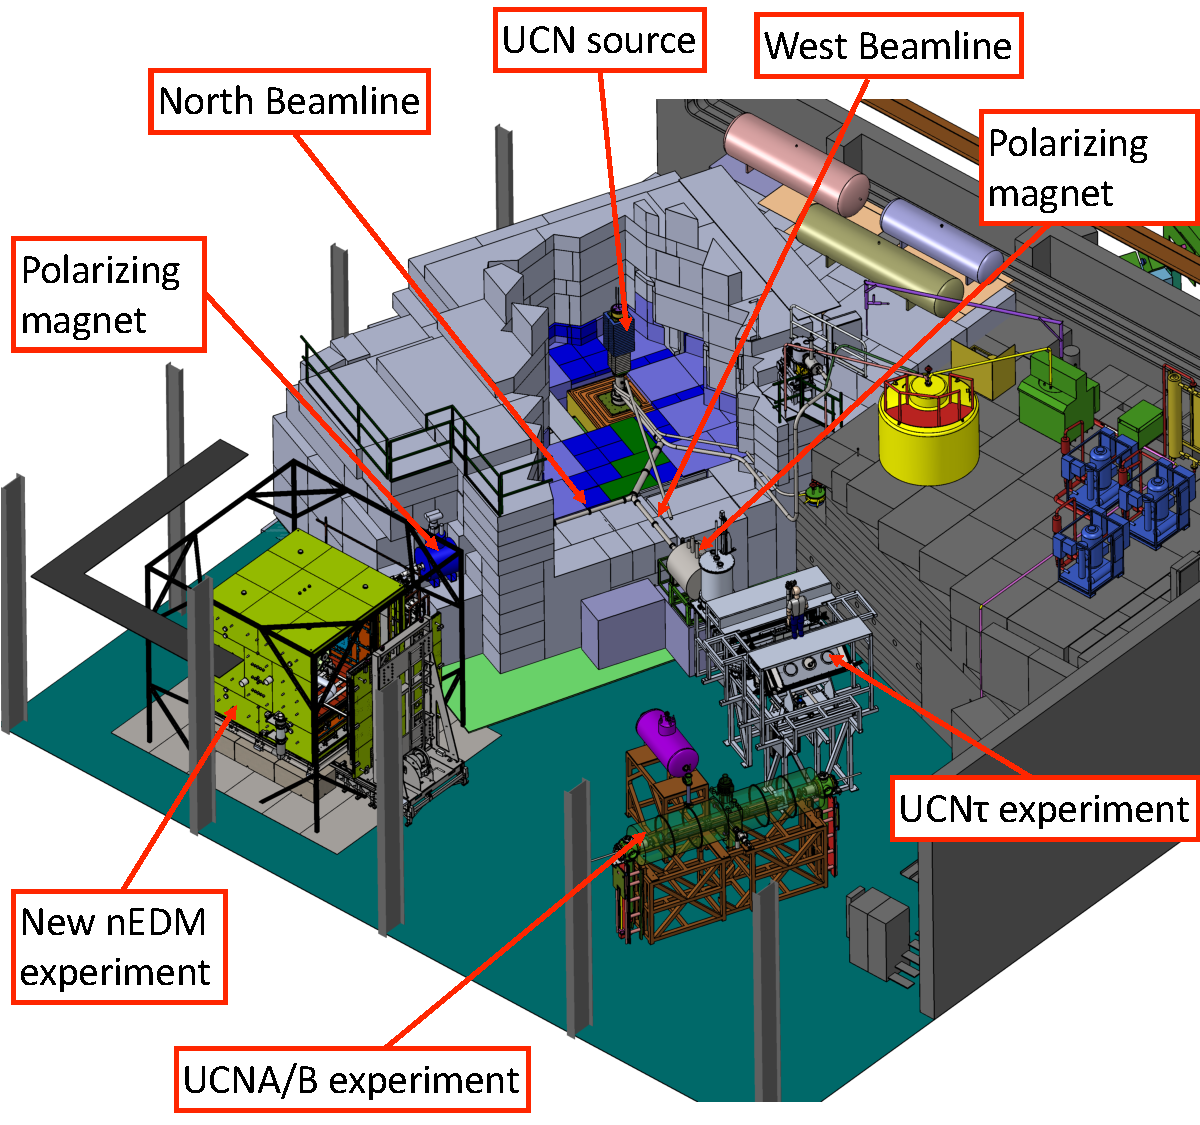
\includegraphics[width=0.6 \textwidth]{AreaB_v3.pdf}
    \caption{Schematic of the experimental area at the LANL UCN facility}
    \label{fig:AreaB_schematic}
\end{figure}

%%%%%%%%%%%%%%%%%%%%%%%%%%%%%%%%%%%%%%%%%

\section{Statistical uncertainty}\label{sec:figure_of_merit}

%%%%%%%%%%%%%%%%%%%%%%%%%%%%%%%%%%%%%%%%%

Equation~7.28 from Ref.~\cite{golubUCN} gives the number of neutrons counted in a single Ramsey sequence as
%
\begin{gather}
    N_\text{R}(\Delta \omega) = N \left( 1 - \gls*{alpha} \cos \,\Delta \omega \, \gls*{T_fp} \right)/2
\end{gather}
%
where \gls*{alpha} is the spin contrast of a Ramsey fringe, defined by Eq.~(\ref{eq:alpha}). \comment{TODO: make sure $T_{fp}$ and $\Delta \omega$ are defined prior}

To maximize sensitivity to small shifts in the resonant frequency, we examine where the slope of the central fringe is largest
%
\begin{gather}
    \frac{\partial N_\text{R}(\Delta \omega)}{\partial \, \Delta \omega} = N \frac{\alpha}{2} \gls*{T_fp} \sin \, \Delta \omega \gls*{T_fp} \label{eq:slope_ramsey}
\end{gather}
%
The error of $\Delta \omega$ is given by
%
\begin{gather}
    \sigma(\Delta \omega) = \frac{\partial \, \Delta \omega}{\partial N_\text{R}(\Delta \omega)}\delta N_\text{R}(\Delta \omega) = \frac{\partial \, \Delta \omega}{\partial N_\text{R}(\Delta \omega)} \sqrt{N}
    \label{eq:sigma_delta_omega}
\end{gather}
%
Using Eq.~(\ref{eq:slope_ramsey}) where $\Delta \omega \, \gls*{T_fp} = \pi/2$ (for the largest slope), Eq.~(\ref{eq:sigma_delta_omega}) becomes
%
\begin{gather}
    \sigma(\Delta \omega) = \frac{2}{\gls*{alpha} \gls*{T_fp} \sqrt{N}}
\end{gather}
%
From reversal of the electric field, we have $\delta \omega_0 = -4 \gls*{d_n} E / \hbar$. \comment{(TODO: derive this eq. earlier (refer to May thesis). define $\omega_0$ as Larmor prec. freq)} This gives
%
\begin{gather}
    \sigma_{\gls*{d_n}} = \frac{\hbar}{2\gls*{alpha} E \gls*{T_fp} \sqrt{N}}\label{eq:figure_of_merit}
\end{gather}
%
This is the figure of merit for an nEDM experiment using the Ramsey method. \gls{hbar} is Planck’s constant, \gls{alpha} is a factor describing the spin contrast of a Ramsey fringe, $N$ is the number of the detected UCN, and $E$ is the strength of the applied electric field.

%%%%%%%%%%%%%%%%%%%%%%%%%%%%%%%%%%%%%%%%%

\subsection
{
    \texorpdfstring{Statistical Uncertainty of the \acrshort{lanl} \acrshort{nedm}}
                    {Statistical Uncertainty of the LANL nEDM}
}

%%%%%%%%%%%%%%%%%%%%%%%%%%%%%%%%%%%%%%%%%

We have demonstrated storage of a sufficient number of polarized UCN to achieve a statistical uncertainty of $\delta \gls*{d_n} = 2\times 10^{-27}$~$e\cdot\text{cm}$ in 5 calendar years of running.

The nominal run parameters for the LANL nEDM are $\gls*{T_fp}=180\text{ s and } E=12\text{ kV/cm}$. As will be shown in Chap.~\ref{chap:north_beamline_paper}, we have measured $N=60\,000\text{ counts per cell}$. We let $\gls*{alpha}=0.8$, as was achieved in Ref.~\cite{ABE20}.

Using Eq.~(\ref{eq:figure_of_merit}), the uncertainty per cell per run is $7.8 \times 10^{-25}e\cdot\text{cm}$. For a full day of measurements (assuming a \qty{300}{\s} duty cycle with two precession cells), we have $N_\text{day}=2\times60\,000\times86\,400\text{ (seconds in a day)}/300$ and $\sigma_{\gls*{d_n}}=3.24\times10^{-26}e\cdot\text{cm}$. A year of continuous running gives $N_\text{year}=365\times N_\text{day}$ and $\sigma_{\gls*{d_n}}=1.7\times10^{-27}e\cdot\text{cm}$. At a 90\% confidence level, the uncertainty is multiplied by an additional factor of $1.6$, giving $\sigma_{\gls*{d_n}}=2.71\times10^{-27}e\cdot\text{cm}$. Accounting for the production schedule at LANL, this uncertainty would be reached in 5 calendar years.

%%%%%%%%%%%%%%%%%%%%%%%%%%%%%%%%%%%%%%%%%

\section
{
    \texorpdfstring{UCN production at \acrshort{lanl}}
                   {UCN production at LANL}
}\label{sec:lanl_ucn_source}

%%%%%%%%%%%%%%%%%%%%%%%%%%%%%%%%%%%%%%%%%

In this upgrade, the cryogenic insert, which houses the SD$_2$ converter as well as the cold neutron moderator, was replaced with an improved design. The upgrade produced a factor of four increase in UCN density~\cite{ito_performance_2018}.

%%%%%%%%%%%%%%%%%%%%%%%%%%%%%%%%%%%%%%%%%

\section
{
    Magnetic field requirements\label{sec:magnetic_field_req}
}

%%%%%%%%%%%%%%%%%%%%%%%%%%%%%%%%%%%%%%%%%


%%%%%%%%%%%%%%%%%%%%%%%%%%%%%%%%%%%%%%%%%

\subsection{Geometric phase}

%%%%%%%%%%%%%%%%%%%%%%%%%%%%%%%%%%%%%%%%%

Rogel eq 6.2.14

%%%%%%%%%%%%%%%%%%%%%%%%%%%%%%%%%%%%%%%%%

\subsection{Magnetically Shielded Room}

%%%%%%%%%%%%%%%%%%%%%%%%%%%%%%%%%%%%%%%%%

%%%%%%%%%%%%%%%%%%%%%%%%%%%%%%%%%%%%%%%%%

\subsection{Performance as a function of ambient temperature}

%%%%%%%%%%%%%%%%%%%%%%%%%%%%%%%%%%%%%%%%%

\comment{Allan Variance}

%%%%%%%%%%%%%%%%%%%%%%%%%%%%%%%%%%%%%%%%%

\subsection{Static and clamped modes of the MSR door}

%%%%%%%%%%%%%%%%%%%%%%%%%%%%%%%%%%%%%%%%%

%%%%%%%%%%%%%%%%%%%%%%%%%%%%%%%%%%%%%%%%%

\subsection{External field active compensation}

%%%%%%%%%%%%%%%%%%%%%%%%%%%%%%%%%%%%%%%%%

%%%%%%%%%%%%%%%%%%%%%%%%%%%%%%%%%%%%%%%%%

\subsection{Transport coils}

%%%%%%%%%%%%%%%%%%%%%%%%%%%%%%%%%%%%%%%%%

%%%%%%%%%%%%%%%%%%%%%%%%%%%%%%%%%%%%%%%%%

\section{Polarizing magnet}\label{sec:PM_description}

%%%%%%%%%%%%%%%%%%%%%%%%%%%%%%%%%%%%%%%%%

%%%%%%%%%%%%%%%%%%%%%%%%%%%%%%%%%%%%%%%%%

\section{Vacuum chamber}

%%%%%%%%%%%%%%%%%%%%%%%%%%%%%%%%%%%%%%%%%

%%%%%%%%%%%%%%%%%%%%%%%%%%%%%%%%%%%%%%%%%

\section{Precession chambers}

%%%%%%%%%%%%%%%%%%%%%%%%%%%%%%%%%%%%%%%%%

%%%%%%%%%%%%%%%%%%%%%%%%%%%%%%%%%%%%%%%%%

\subsection{dPS coating procedure}

%%%%%%%%%%%%%%%%%%%%%%%%%%%%%%%%%%%%%%%%%



%%%%%%%%%%%%%%%%%%%%%%%%%%%%%%%%%%%%%%%%%

\section{Spin flipper and analyzers}\label{sec:spin_flipper_analyzer}

%%%%%%%%%%%%%%%%%%%%%%%%%%%%%%%%%%%%%%%%%

%%%%%%%%%%%%%%%%%%%%%%%%%%%%%%%%%%%%%%%%%

\section{Scanning for magnetic contamination}

%%%%%%%%%%%%%%%%%%%%%%%%%%%%%%%%%%%%%%%%%